\section{Activity Diagrams}

Primary path analysis ensures that the exceptional and common paths throughout 
a system are identified \citep{lunn03}. Activity diagrams take these paths and
break them up into easy to follow, manageable processes.

An activity is a task in a process that allows for small meaningful work to 
happen. A process may have a number of activities linked together to form a 
work flow \citep{lunn03}.

\subsection{Import KML}
Figure \ref{fig:importkmlactivity} illustrates the simple action of importing 
the KML file into the system. In order to obtain the values from the file, a 
KML parser (or more precisely an XML Parser) is required. 

The parser will attempt to read each `Placemark' found within the file, and 
will try to read any additional meta data supplied.

Each placemark tag will be required to be converted to an Event object, so that 
the Events can be clustered.

\begin{figure}[H]
  \centering
    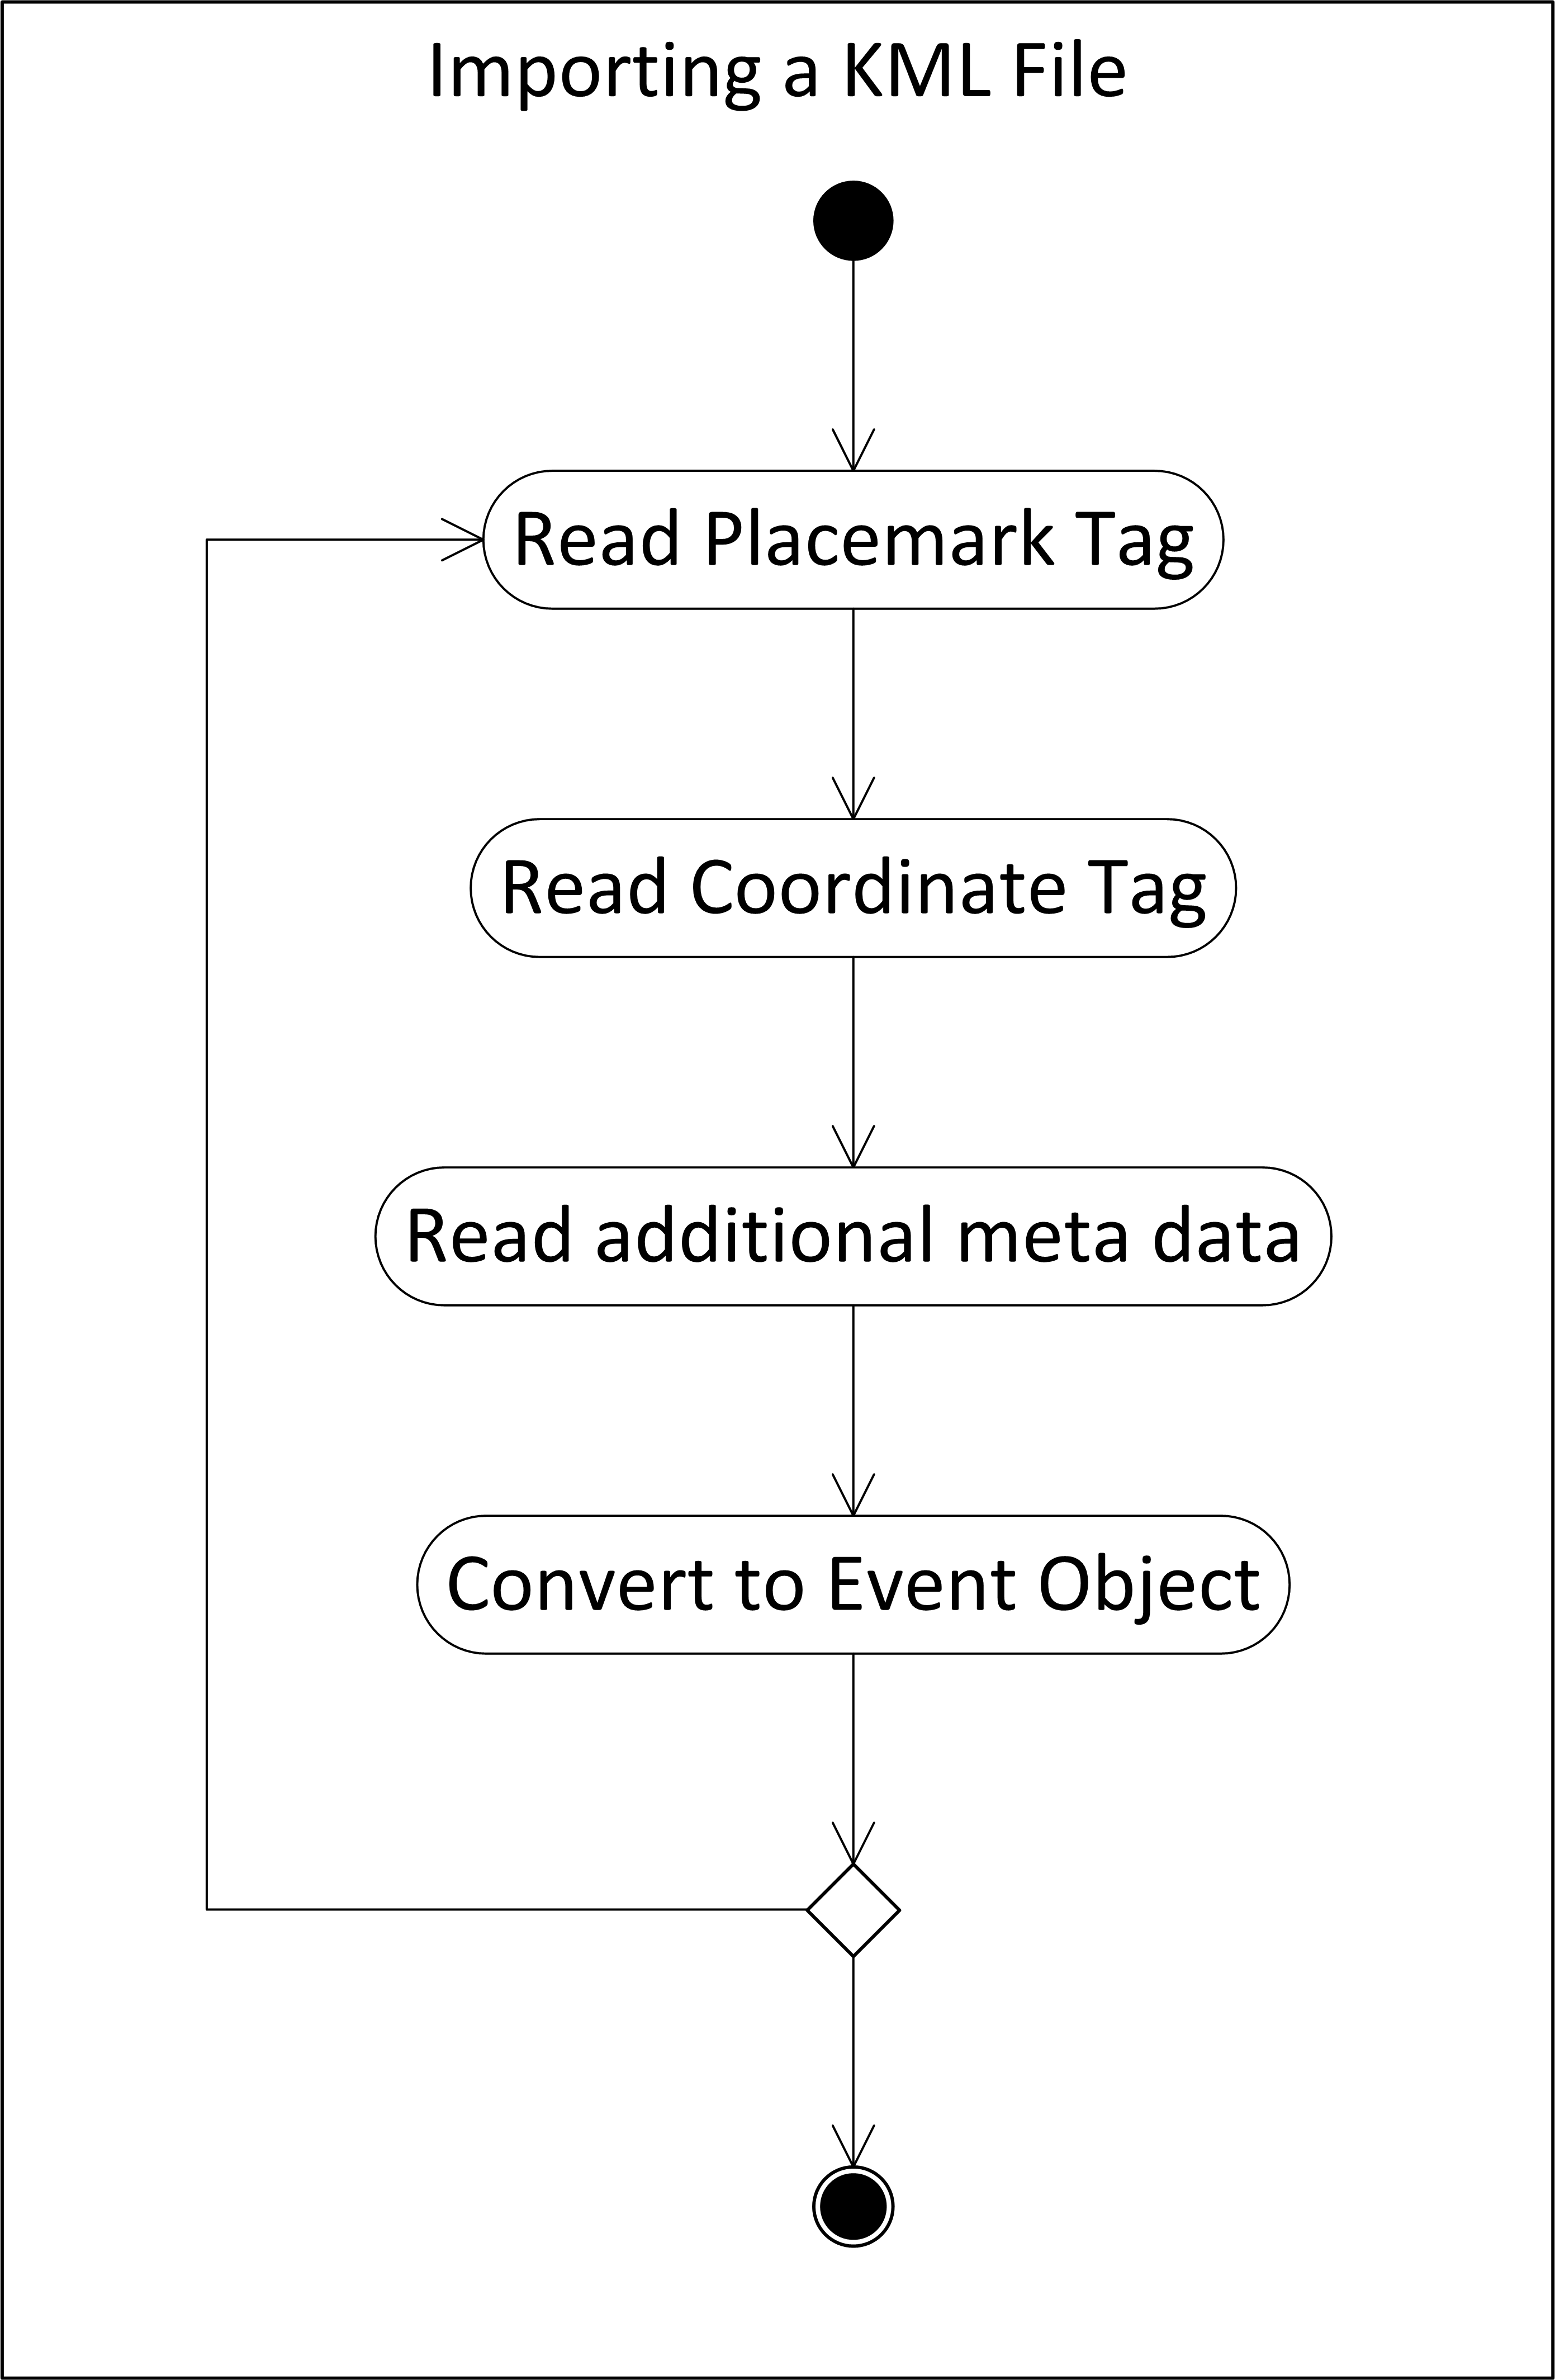
\includegraphics[scale=0.6]{chapter7/activity/import_kml.png}
    \caption[Importing a KML File activity diagram]
            {An activity digram highlighting the various actions that are 
             required to be taken in order to import a KML file}
    \label{fig:importkmlactivity}
\end{figure}


\subsection{Cluster Data}
Figure \ref{fig:clusterdataactivity} highlights the activity for clustering a 
set of Events using the DBSCAN algorithm. 

The algorithm will visit all points within the dataset, and for each 
unvisited point a neighbourhood visit will occur.

This means that the intra-cluster similarity will be calculated, and if it is 
deemed that two objects are related they will be placed into the same cluster.

All points that are deemed to be noise, will be separated from the resulting 
clusters. A noise point is one that does not fit into the neighbourhood of 
another point.

Border points are assigned upon the fly (rather than at the end of the 
clustering process) based upon the cluster that they are the closest to. The 
distance is based upon the centroid of the cluster (average of all objects 
within a cluster).

\begin{figure}[H]
  \centering
    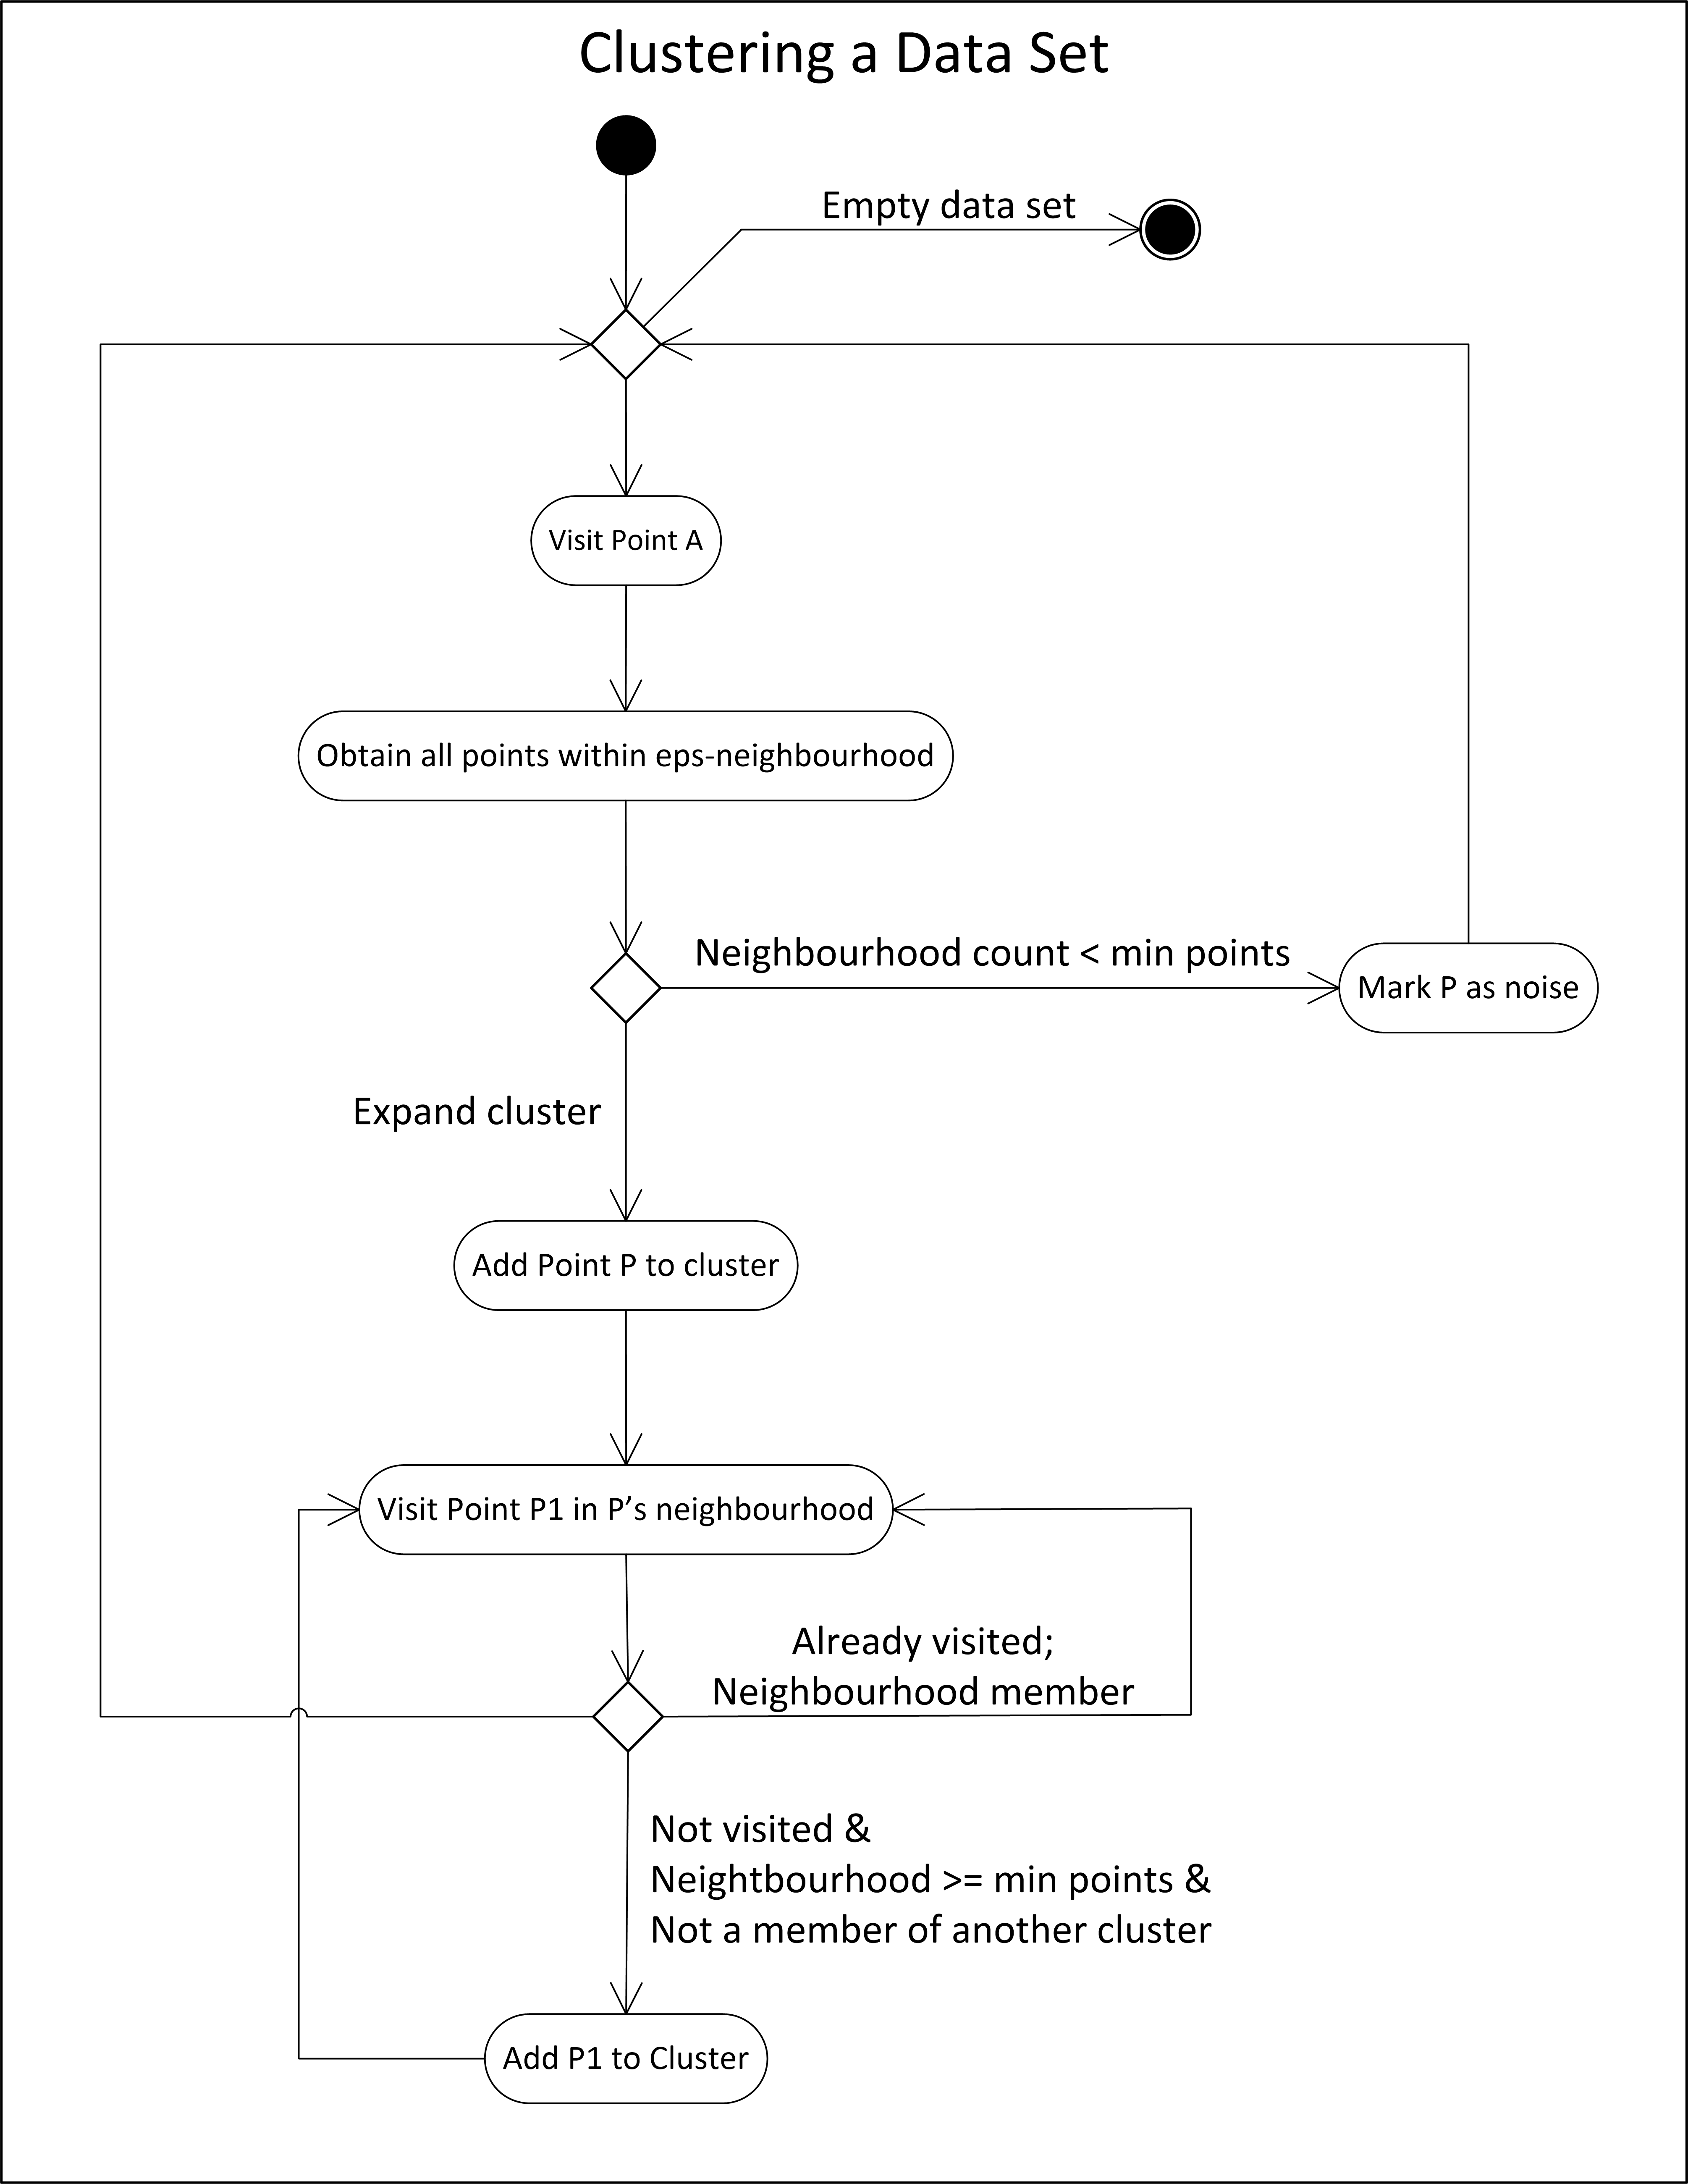
\includegraphics[scale=0.7]{chapter7/activity/clustering_data_set.png}
    \caption[Clustering a data set activity diagram]
            {An activity digram highlighting the various actions that are 
             required to be taken in order to cluster a set of data}
    \label{fig:clusterdataactivity}
\end{figure}



\subsection{Analysing a Cluster}
Figure \ref{fig:analyseclusteractivity} highlights the analysis of a cluster. 
This activity performs a number of business actions, that have been defined 
directly by BlackBerry. Identification of the cluster sizes, the similarities 
and differences form part of the first initial points to start to analyse the 
clusters.

Once completed, a more in depth analysis takes place. This in depth analysis 
looks at differences between the meta data (additional data associated with an 
Event), such as the RAT usage.

\begin{figure}[H]
  \centering
    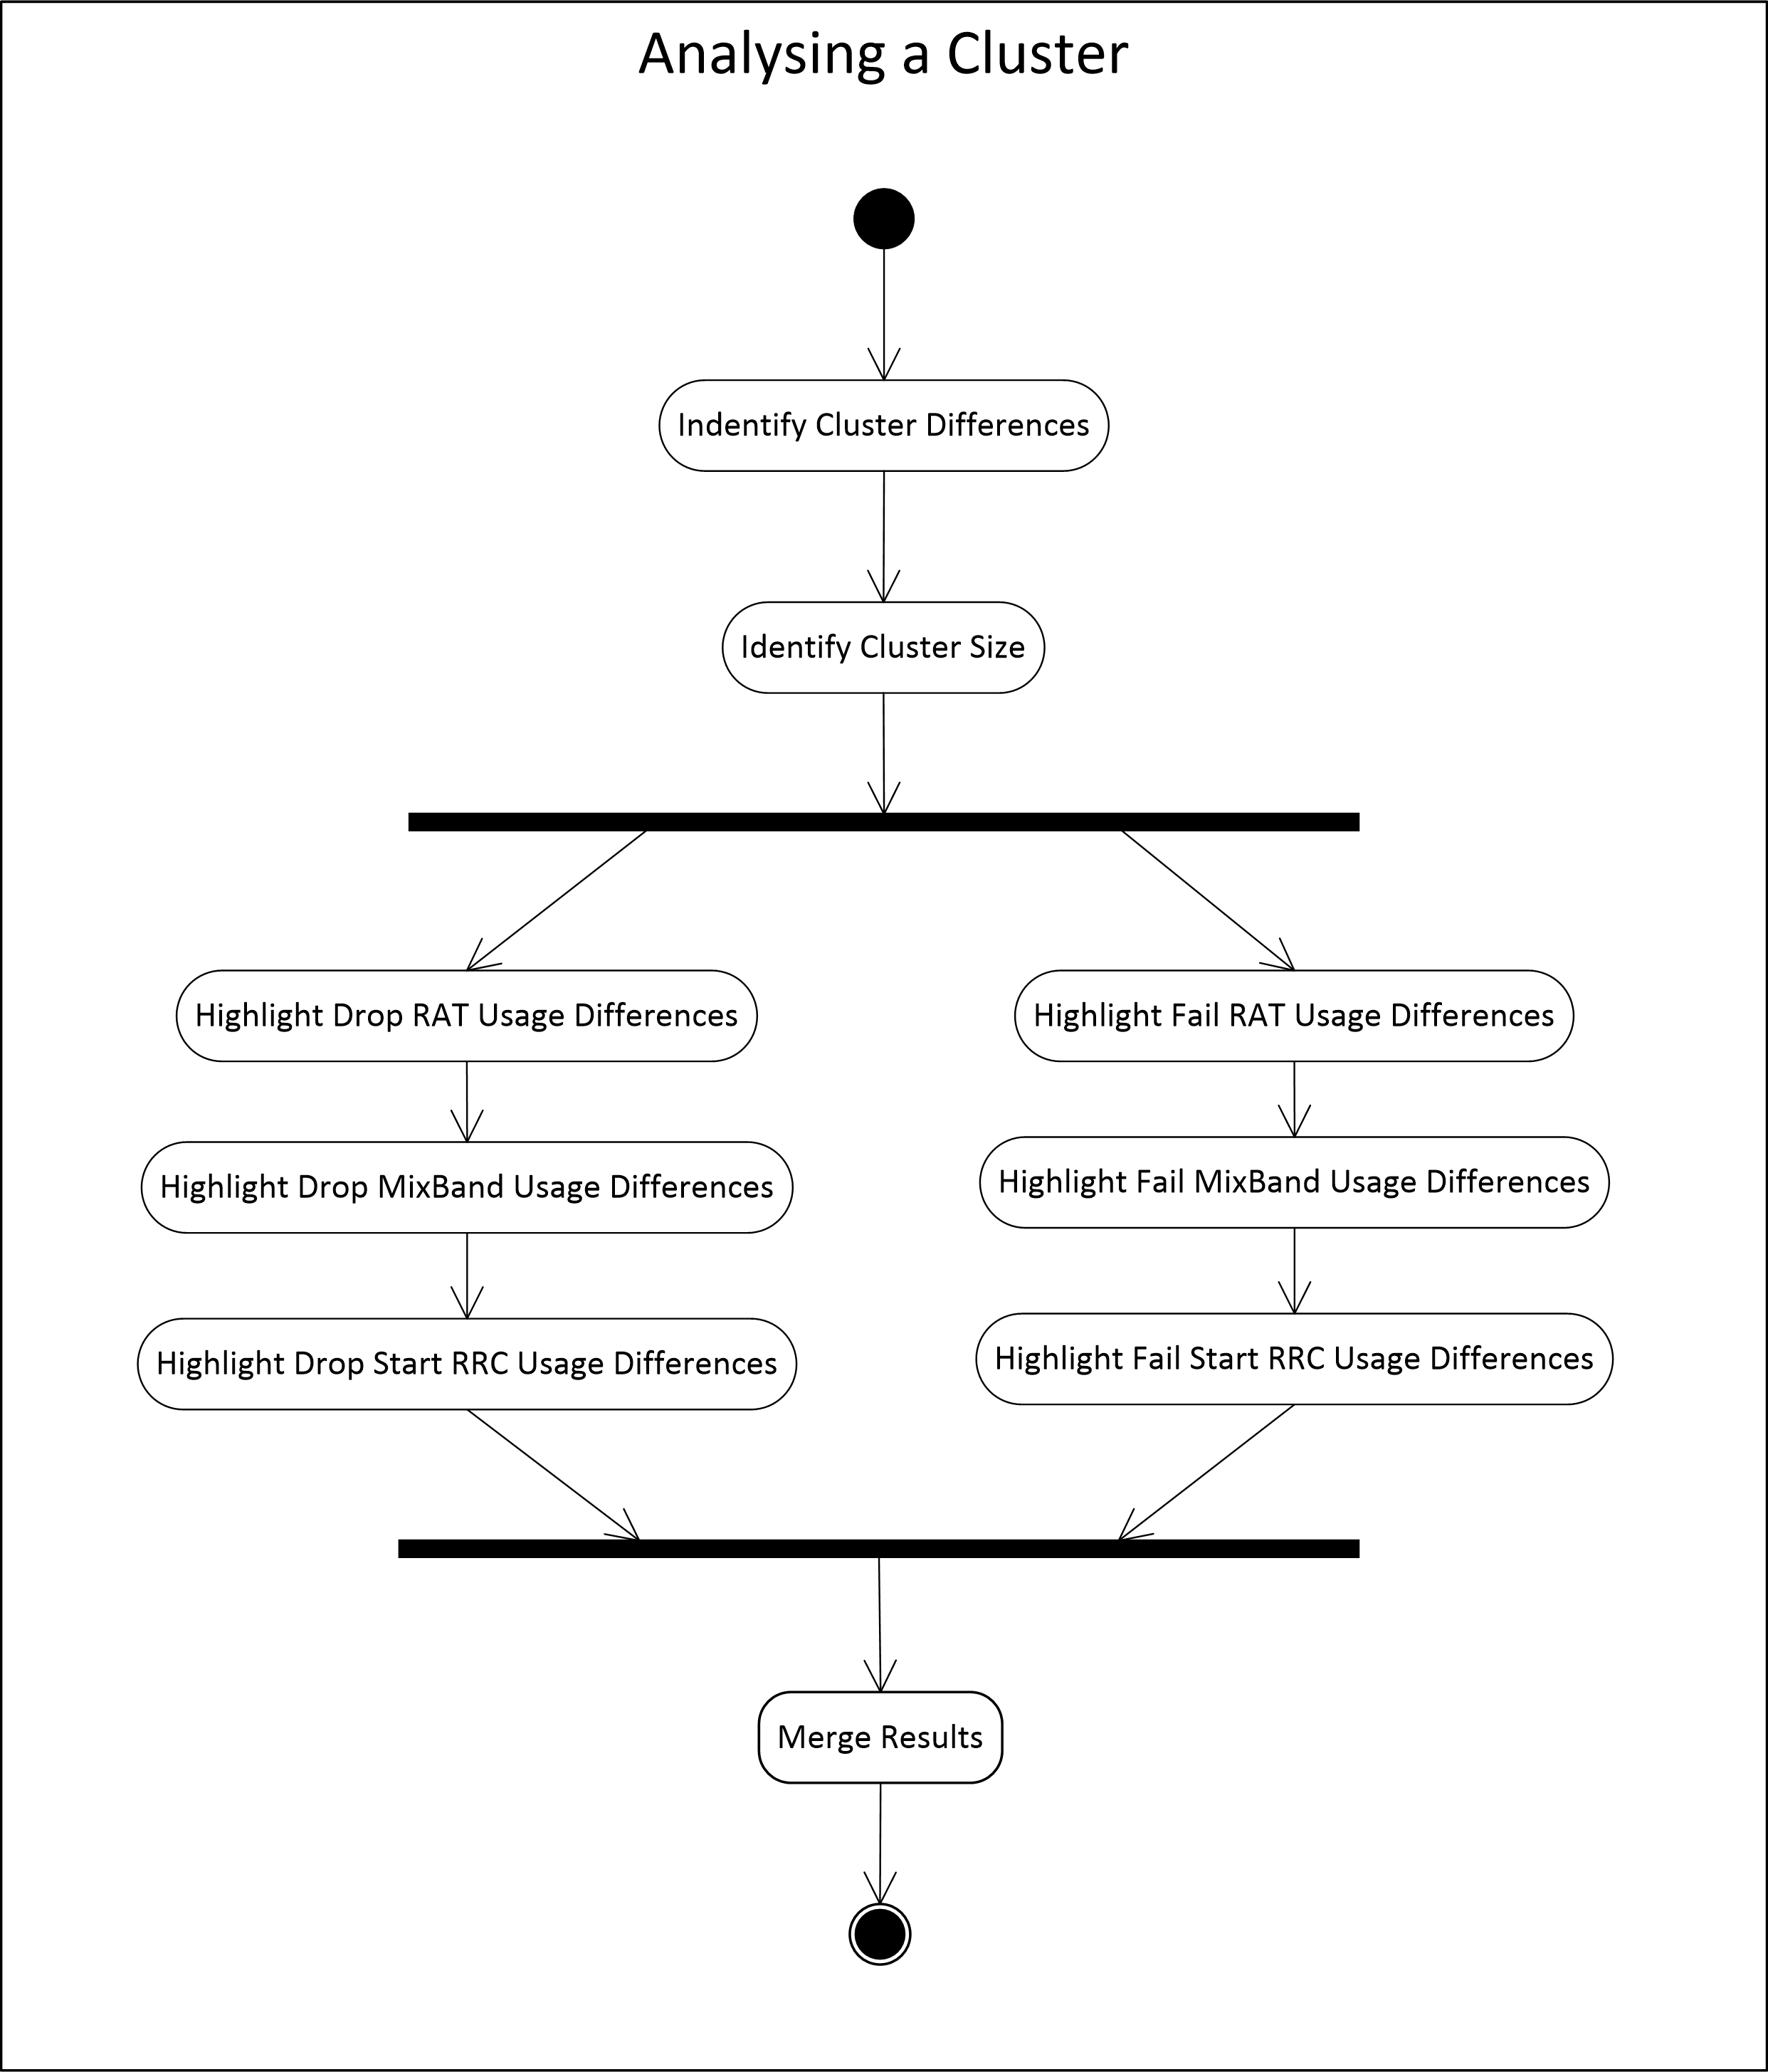
\includegraphics[scale=0.6]{chapter7/activity/analyse_cluster.png}
    \caption[Analysing a cluster activity diagram]
            {An activity digram highlighting the various actions that are 
             required to be taken in order analyse a clustered set of data}
    \label{fig:analyseclusteractivity}
\end{figure}
